\section{Kiến trúc Hệ thống và Mô hình hóa Toán học Chi tiết}

\subsection{Hình thức hóa Bài toán Ghép cặp Hai chiều}
Ký hiệu $\mathcal{D}$ là không gian toàn thể các tài liệu tuyển dụng, được phân hoạch thành tập mô tả công việc $\mathcal{J}$ và tập hồ sơ ứng viên $\mathcal{C}$. Trong kịch bản ghép cặp tổng quát, cho trước một tài liệu truy vấn $D_q \in \mathcal{D}$ (khi tuyển dụng: $D_q \in \mathcal{J}$; khi gợi ý việc làm: $D_q \in \mathcal{C}$) và một tập ứng viên rút gọn $\mathcal{C}_{cand} = \{D_1, D_2, \dots, D_N\}$ gồm $N$ tài liệu đối sánh. Mỗi cặp truy vấn--ứng viên $(D_q, D_i)$ sở hữu một mức độ phù hợp thực tế (ground-truth relevance grade) ký hiệu là $y_{q, i} \in \{0, 1, 2, 3\}$, tương ứng với các mức: Không phù hợp ($0$), Phù hợp một phần ($1$), Phù hợp tốt ($2$), và Phù hợp xuất sắc ($3$).

Mục tiêu của hệ thống xếp hạng là tìm ra một hoán vị thứ tự $\pi^*$ trên tập chỉ số $\{1, 2, \dots, N\}$ sao cho tối đa hóa chỉ số nDCG@K (Normalized Discounted Cumulative Gain tại ngưỡng $K$):
\begin{equation}
    \pi^* = \arg\max_{\pi} \text{nDCG}@K\big( \pi(\mathcal{C}_{cand}), \mathbf{y}_q \big).
    \label{eq:objective}
\end{equation}

\begin{figure}[t]
\centering
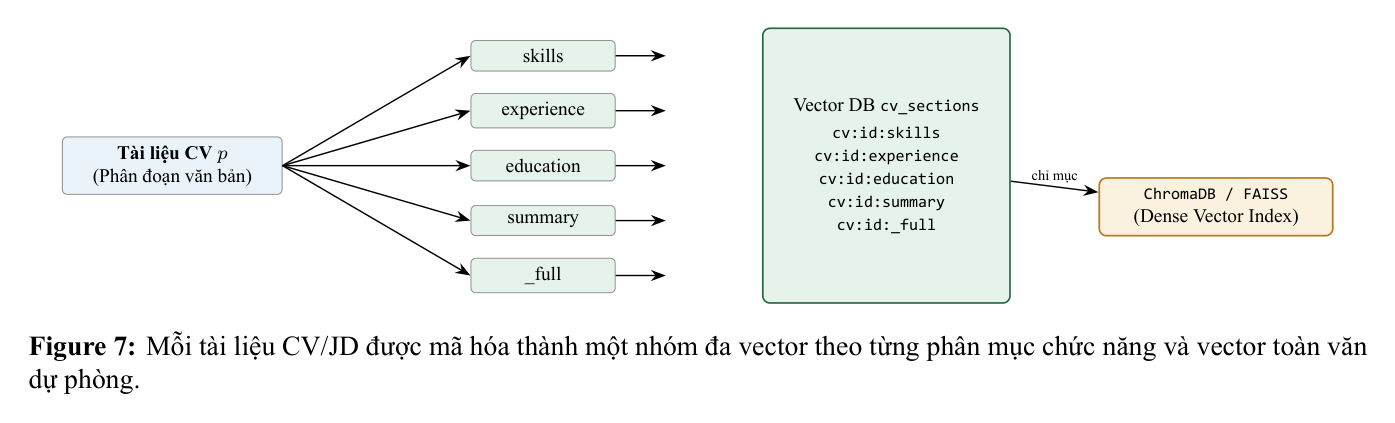
\includegraphics[width=0.88\textwidth]{figures/fig07_vector_theo_section.png}
\caption{Kiến trúc biểu diễn đa vector nhận biết phân mục và cơ chế căn chỉnh chéo giữa Mô tả Công việc (JD) và Hồ sơ Ứng viên (CV).}
\label{fig:arch}
\end{figure}

Kiến trúc tổng thể của hệ thống được minh họa trên Hình~\ref{fig:arch}, tách biệt thành hai luồng xử lý độc lập:
\begin{itemize}
    \item \textbf{Luồng Ngoại tuyến (Offline Indexing Pipeline)}: Trích xuất siêu dữ liệu, phân đoạn văn bản thô thành các phân mục chức năng thông qua bộ bóc tách quy tắc tất định, tạo các biểu diễn vector đặc thông qua mô hình Bi-Encoder đóng băng, và cập nhật chỉ mục cơ sở dữ liệu vector ChromaDB bất đồng bộ.
    \item \textbf{Luồng Trực tuyến (Online Serving Pipeline)}: Tiếp nhận truy vấn trong thời gian thực, tính toán ma trận tương đồng ghép chéo giữa các phân mục, thực thi tái chuẩn hóa trọng số động, hợp nhất điểm xếp hạng lai hai tầng và xuất giải thích minh bạch (Grounded Explanation).
\end{itemize}

\subsection{Thuật toán Bóc tách Phân mục Quy tắc Không Rò rỉ}
Khác với các phương pháp nén văn bản mù, hệ thống bóc tách mỗi tài liệu $D$ thành một tập hợp gồm $M$ phân mục chức năng có tên gọi rõ ràng:
\begin{equation}
    D = \Big\{ \big(s_1, T_1\big), \big(s_2, T_2\big), \dots, \big(s_M, T_M\big), \big(\text{full}, T_{raw}\big) \Big\},
\end{equation}
trong đó mỗi nhãn phân mục $s_m \in \mathcal{S}_{domain} = \{\text{skills}, \text{experience}, \text{education}, \text{summary}, \text{projects}\}$, và $T_m$ là chuỗi ký tự nội dung tương ứng của mục đó; $T_{raw}$ là toàn văn tài liệu gốc.

Bộ bóc tách phân mục (Section Parser, mã băm commit \texttt{41e1d27}) vận hành hoàn toàn theo quy tắc biểu thức chính quy (Regex) với ranh giới từ (\texttt{\textbackslash b}), kết hợp từ điển mở rộng gồm hơn $40$ biến thể tiêu đề chuẩn mực (ví dụ: đối với mục kinh nghiệm làm việc: \texttt{work experience}, \texttt{professional experience}, \texttt{employment history}, \texttt{career history}). Nhằm giải quyết triệt để lỗi dính chữ trong các tài liệu trích xuất từ định dạng HTML/PDF (ví dụ: \texttt{EducationGMR Institute} hoặc \texttt{ExperienceSoftware Engineer}), bộ tách áp dụng quy tắc nhận diện ranh giới ký tự viết hoa đứng liền sau chữ thường:
\begin{equation}
    \text{Pattern}_{\text{split}} = \text{\texttt{r'(?<=[a-z])(?=[A-Z][a-z]+)'}}.
\end{equation}

Toàn bộ quá trình hiệu chỉnh biểu thức chính quy được thực hiện nghiêm ngặt trên tập phát triển nội bộ (\texttt{train\_dev}, 204 JD), tuyệt đối không tiếp xúc với tập đánh giá độc lập (\texttt{train\_clean}, 76 JD) hay tập kiểm thử chính thức (\texttt{test}, 71 JD). Khi một tài liệu hoàn toàn không chứa bất kỳ tiêu đề phân mục nào nhận diện được, cơ chế dự phòng an toàn (Fallback Mechanism) sẽ tự động gán toàn văn $T_{raw}$ vào phân mục giả định \texttt{full}, đảm bảo hệ thống không bao giờ bị gián đoạn hay sinh lỗi ngoại lệ trong luồng vận hành.

\subsection{Biểu diễn Đa Vector Độc lập}
Sau khi văn bản được phân đoạn, mỗi đoạn văn bản phân mục $T_m$ cũng như toàn văn $T_{raw}$ được đưa qua mô hình Bi-Encoder hai nhánh đóng băng $\mathcal{E}(\cdot)$ (trong nghiên cứu này sử dụng \texttt{all-MiniLM-L6-v2} với số chiều $d=384$ hoặc \textsc{BAAI/bge-m3} với $d=1024$) để tạo ra vector đặc tương ứng:
\begin{equation}
    \mathbf{v}_m = \mathcal{E}(T_m) \in \mathbb{R}^d, \quad \mathbf{v}_{full} = \mathcal{E}(T_{raw}) \in \mathbb{R}^d.
\end{equation}
Mỗi vector đầu ra được chuẩn hóa theo chuẩn Euclid ($L_2$-norm) về độ dài đơn vị:
\begin{equation}
    \mathbf{v} \leftarrow \frac{\mathbf{v}}{\|\mathbf{v}\|_2} = \frac{\mathbf{v}}{\sqrt{\sum_{i=1}^d v_i^2}}, \quad \text{sao cho } \|\mathbf{v}\|_2 = 1.
\end{equation}
Nhờ chuẩn hóa $L_2$, tích vô hướng giữa hai vector $\mathbf{u} \cdot \mathbf{w} = \sum_{i=1}^d u_i w_i$ chính là độ tương đồng Cosine:
\begin{equation}
    \text{sim}(\mathbf{u}, \mathbf{w}) = \cos(\theta) = \frac{\mathbf{u} \cdot \mathbf{w}}{\|\mathbf{u}\|_2 \|\mathbf{w}\|_2} = \mathbf{u} \cdot \mathbf{w} \in [-1, 1].
\end{equation}

\subsection{Ghép cặp Chéo và Tái Chuẩn hóa Trọng số Động}
Trong các CV thực tế, kỹ năng chuyên môn thường không được liệt kê tập trung trong một mục riêng biệt mà nằm rải rác trong phần mô tả dự án hoặc quá trình công tác. Nếu chỉ ghép cặp cứng các mục có cùng tên (Fixed Same-Name Matching), hệ thống sẽ đánh mất các kỹ năng ẩn này. Do đó, chúng tôi áp dụng cơ chế \textbf{Ghép cặp Chéo Mục (Cross-Section Pairing)}: mỗi phân mục $s_m$ trong tài liệu truy vấn $D_q$ sẽ được tìm kiếm phân mục có độ tương đồng ngữ nghĩa lớn nhất trên toàn bộ các phân mục hiện diện trong tài liệu ứng viên $D_c$:
\begin{equation}
    c(s_m) = \max_{s_k \in \mathcal{S}(D_c)} \text{sim}\big(\mathbf{v}_q^{s_m}, \mathbf{v}_c^{s_k}\big).
    \label{eq:cross_pairing}
\end{equation}

Trong các hồ sơ ứng viên mới tốt nghiệp hoặc vị trí việc làm tự do ngắn hạn, một số phân mục tự chọn (như dự án hay bằng cấp học vấn) thường bị khuyết thiếu. Việc gán giá trị 0 cố định cho các mục thiếu sẽ trừng phạt bất công các ứng viên đủ năng lực. Để giải quyết vấn đề này, chúng tôi thiết lập cơ chế \textbf{Tái Chuẩn hóa Trọng số Động (Dynamic Weight Renormalization)}:
\begin{equation}
    S_{sem}(D_q, D_c) = \frac{\sum_{m \in \mathcal{S}_{\text{matched}}} w_m \cdot c(s_m)}{\sum_{m \in \mathcal{S}_{\text{matched}}} w_m},
    \label{eq:dynamic_renorm}
\end{equation}
trong đó $\mathcal{S}_{\text{matched}} = \mathcal{S}(D_q) \cap \mathcal{S}_{\text{active}}$ là tập các phân mục thực sự hiện diện trong truy vấn, và $w_m$ là trọng số cơ sở được ấn định theo tri thức nghiệp vụ tuyển dụng (commit \texttt{55c22ae}):
\begin{itemize}
    \item $w_{\text{skills}} = 0.40$ (hoặc $0.35$ khi có mục tóm tắt): Kỹ năng kỹ thuật cốt lõi là điều kiện tiên quyết quyết định ứng viên có thể thực hiện công việc hay không, do đó mang trọng số cao nhất.
    \item $w_{\text{exp}} = 0.35$: Kinh nghiệm thực chiến chứng minh năng lực áp dụng lý thuyết vào bối cảnh thực tế và giải quyết vấn đề.
    \item $w_{\text{proj}} = 0.15$: Dự án cá nhân và sản phẩm thực tế là minh chứng bổ trợ cho năng lực tự học và đam mê chuyên môn.
    \item $w_{\text{edu}} = 0.10$: Nền tảng học thuật là điều kiện nền tảng nhưng ít tính phân hóa hơn kinh nghiệm thực tế trong thị trường việc làm tự do.
\end{itemize}
Mẫu số $\sum_{m \in \mathcal{S}_{\text{matched}}} w_m$ đảm bảo tổng trọng số hiệu dụng sau khi tái chuẩn hóa luôn đúng bằng $1.0$, giữ cho thang đo điểm số $S_{sem} \in [0, 1]$ được ổn định tuyệt đối giữa mọi cặp tài liệu.

\subsection{Động cơ Xếp hạng Lai Hai Tầng}
Nhằm đảm bảo sự tách biệt rành mạch giữa các ràng buộc pháp lý/nghiệp vụ và năng lực chuyên môn, hệ thống vận hành theo kiến trúc hai tầng:
\begin{itemize}
    \item \textbf{Tầng 1: Bộ lọc Ràng buộc Tiên quyết (Eligibility Hard Filters)}: Loại bỏ các ứng viên không thỏa mãn điều kiện thị trường không liên quan đến năng lực (tài khoản không hoạt động, vi phạm chính sách quyền riêng tư, không sẵn sàng nhận việc, hoặc kỳ vọng ngân sách vượt quá trần chi trả của dự án).
    \item \textbf{Tầng 2: Điểm Xếp hạng Năng lực Lai (Unified Competency Scoring)}: Các ứng viên vượt qua Tầng 1 được tính điểm thông qua phương trình hợp nhất:
    \begin{equation}
        S_{hybrid}(c, j) = \alpha \cdot S_{sem}^{\text{norm}}(c, j) + (1 - \alpha) \cdot S_{lex}^{\text{norm}}(c, j) + \beta \cdot S_{tax}(c, j),
        \label{eq:hybrid_full}
    \end{equation}
    trong đó các điểm thành phần được chuẩn hóa tuyến tính Min-Max về khoảng $[0, 1]$ trên tập kết quả của từng truy vấn:
    \begin{equation}
        S^{\text{norm}}(c, j) = \frac{S(c, j) - \min_{k} S(k, j)}{\max_{k} S(k, j) - \min_{k} S(k, j) + \epsilon}, \quad (\epsilon = 10^{-8}).
    \end{equation}
\end{itemize}

\noindent\textbf{Ý nghĩa của các Hằng số Điều phối}:
\begin{itemize}
    \item $\alpha = 0.60$: Trọng số ưu tiên phân bổ $60\%$ cho độ tương đồng ngữ nghĩa đặc ($S_{sem}$) nhằm nắm bắt ngữ cảnh trừu tượng và thuật ngữ tương đương, và dành $40\%$ ($1 - \alpha = 0.40$) cho điểm từ vựng BM25 ($S_{lex}$) nhằm bảo đảm tính chính xác từng chữ đối với các tên thư viện và công nghệ hiếm.
    \item $\beta = 0.60$: Hệ số điều phối tỷ trọng đóng góp của độ phủ kỹ năng cấu trúc từ cây phân loại ($S_{tax}$) khi kết hợp vào điểm tổng thể, được hiệu chuẩn dựa trên tập huấn luyện nội bộ nhằm đạt mức tương quan thứ hạng cao nhất.
\end{itemize}

\subsection{Xếp hạng Phối hợp Nghịch đảo Không Tham số (Parameter-Free RRF)}
Để loại bỏ nguy cơ quá khớp (overfitting) do việc dò tìm các siêu tham số $\alpha, \beta$, chúng tôi cung cấp giải pháp thay thế dựa trên thuật toán Reciprocal Rank Fusion (RRF) \cite{cormack2009reciprocal}:
\begin{equation}
    S_{RRF}(d) = \sum_{m \in \mathcal{M}} \frac{1}{k + r_m(d)},
    \label{eq:rrf}
\end{equation}
trong đó $\mathcal{M} = \{\text{Dense}, \text{BM25}\}$ là tập các danh sách xếp hạng thành phần, $r_m(d) \in \{1, 2, \dots, N\}$ là vị trí thứ hạng của tài liệu $d$ trong danh sách $m$, và $k = 60$ là hằng số làm mịn kinh điển theo chuẩn quốc tế. Hằng số $k=60$ có vai trò ngăn ngừa việc một ứng viên đứng đầu ở một danh sách thành phần duy nhất lấn át hoàn toàn các ứng viên có vị trí cao đồng đều ở cả hai danh sách.

\subsection{Độ phủ Kỹ năng Bất đối xứng trên Cây Phân loại 3 Tầng}
Thay vì áp dụng công thức tương đồng Jaccard đối xứng truyền thống vốn trừng phạt bất công các ứng viên sở hữu nhiều kỹ năng phong phú vượt ngoài mô tả công việc, thành phần $S_{tax}$ đo lường mức độ đáp ứng kỹ năng theo hướng bất đối xứng một chiều ($\text{JD} \rightarrow \text{CV}$):
\begin{equation}
    \text{Cov}(\mathcal{T}) = \frac{\sum_{t \in \mathcal{T}} \mathbb{I}(t \in \mathcal{C}_{skills}) \cdot w_t}{\sum_{t \in \mathcal{T}} w_t},
\end{equation}
trong đó $\mathcal{T}$ là tập hợp các kỹ năng được trích xuất từ bài đăng tuyển dụng, $\mathcal{C}_{skills}$ là tập kỹ năng của ứng viên sau khi đã mở rộng qua cây phân loại (bao gồm các từ đồng nghĩa Tầng 1 và quan hệ phân cấp cha-con Tầng 2, ví dụ: \texttt{PyTorch} $\implies$ \texttt{Deep Learning}), và $w_t$ là trọng số mức độ quan trọng của kỹ năng $t$.

Điểm kỹ năng tổng hợp phân biệt rõ ràng giữa hai nhóm tiêu chí:
\begin{equation}
    S_{skills} = 0.8 \cdot \text{Cov}(\text{MustHave}) + 0.2 \cdot \text{Cov}(\text{NiceToHave}).
    \label{eq:must_nice}
\end{equation}
Tỷ lệ $80/20$ ($0.8$ cho Must-Have và $0.2$ cho Nice-To-Have) phản ánh đúng thực tế tuyển dụng: một ứng viên chỉ có thể được xem xét nếu đáp ứng phần lớn các điều kiện tiên quyết. Đặc biệt, nếu ứng viên đáp ứng dưới $50\%$ số kỹ năng bắt buộc ($\text{Cov}(\text{MustHave}) < 0.50$), hệ thống kích hoạt hệ số phạt nhân tử:
\begin{equation}
    \gamma = \text{Cov}(\text{MustHave}), \quad S_{skills} \leftarrow S_{skills} \cdot \gamma,
\end{equation}
ngăn chặn triệt để hiện tượng ứng viên bù đắp thiếu hụt kỹ năng sống còn bằng cách tích lũy nhiều kỹ năng phụ không quan trọng.

Bảng~\ref{tab:design_decisions} tổng hợp toàn bộ các quyết định thiết kế kiến trúc, giải pháp thay thế và bằng chứng thực nghiệm của hệ thống.

% Bảng quyết định thiết kế kiến trúc, phương án thay thế và bằng chứng thực nghiệm
\begin{table*}[t]
\centering\small
\caption{Các quyết định thiết kế hệ thống, giải pháp thay thế, lý do kiến trúc và bằng chứng thực nghiệm.}
\label{tab:design_decisions}
\resizebox{\textwidth}{!}{%
\begin{tabular}{@{}llll@{}}
\toprule
\textbf{Quyết định thiết kế} & \textbf{Giải pháp thay thế} & \textbf{Lý do kiến trúc} & \textbf{Bằng chứng thực nghiệm} \\ \midrule
\textbf{Phân mảnh Đa Vector} & Đơn Vector phẳng / Chunking & Tránh loãng ngữ nghĩa các kỹ năng hiếm & Ngăn chặn hiện tượng cắt ngắn văn bản ($>95\%$ tránh truncation) \\
\textbf{Ghép cặp Chéo Mục} & Ghép cặp cứng cùng tên mục & Khai thác kỹ năng lồng trong kinh nghiệm & Bao phủ thông tin khi $26\%$ CV thiếu tiêu đề kỹ năng riêng \\
\textbf{Tái chuẩn hóa Trọng số} & Gán điểm 0 cho mục thiếu & Tránh phạt bất công hồ sơ mới tốt nghiệp & Giữ chuẩn hóa điểm số công bằng giữa các loại ứng viên \\
\textbf{Độ phủ Kỹ năng Bất đối xứng} & Jaccard Đối xứng & Đo lường mức độ đáp ứng yêu cầu tuyển dụng & Phân biệt rõ kỹ năng bắt buộc (Must) và ưu tiên (Nice) \\
\textbf{Tìm kiếm Lai Hai Tầng} & Quét thô toàn bộ ứng viên & Đạt độ trễ trực tuyến thời gian thực & $T_{\text{rank}} = 2.69$\,ms cho pool $N=25$ ứng viên trên CPU \\
\textbf{Giải thích Minh bạch Căn cứ} & Mô hình Sinh LLM Hộp đen & Trích xuất trực tiếp bằng chứng từ điểm số & Loại bỏ hiện tượng ảo giác, hỗ trợ giải trình pháp lý \\ \bottomrule
\end{tabular}%
}
\end{table*}

